\documentclass[11pt,conference,draftcls,onecolumn]{IEEEtran}
\pagestyle{plain}
\IEEEoverridecommandlockouts
% The preceding line is only needed to identify funding in the first footnote. If that is unneeded, please comment it out.
\usepackage{cite}
\usepackage{amsmath,amssymb,amsfonts}
\usepackage{algorithmic}
\usepackage{graphicx}
\usepackage{textcomp}
\usepackage{xcolor}
\usepackage{listings}
\def\BibTeX{{\rm B\kern-.05em{\sc i\kern-.025em b}\kern-.08em
    T\kern-.1667em\lower.7ex\hbox{E}\kern-.125emX}}
\begin{document}

\title{Online Anomaly Detection in Request-Based Battery Management Systems\\
{}
\thanks{This work was funded in part by NSF Grant No. 1234567}
}

\author{\IEEEauthorblockN{Aaron Willcock}
\IEEEauthorblockA{\textit{Department of Computer Science} \\
\textit{Wayne State University}\\
Detroit, MI, USA \\
aaron.willcock@wayne.edu}
\and
\IEEEauthorblockN{Nathan Fisher}
\IEEEauthorblockA{\textit{Department of Computer Science} \\
\textit{Wayne State University}\\
Detroit, MI, USA \\
fishern@wayne.edu}
}

\maketitle

\begin{abstract}
Battery Management System (BMS) research has included reconfigurable cell architecture, state of health estimation, battery balancing, and real-time scheduling.
However, anomaly detection in BMSs is addressed only as an offline method for identifying malfunctions or parasitic loads.
Furthermore, the costly implementation of BMSs has resulted in few works evaluating approaches outside of simulation.
In this report, a low-cost BMS is designed and implemented with an online anomaly detection system to mitigate damage in real-time.   
\end{abstract}

\begin{IEEEkeywords}
battery management system, anomaly detection, real-time systems
\end{IEEEkeywords}

\section{Introduction}
The number of plug-in electric vehicles (hybrid and pure-electric) is expected to reach over 70 million by 2030 according to the International Energy Agency \cite{iea}.
Electric vehicles typically contain a Battery Management System (BMS) responsible for handling the charging, discharging, reconfiguration, monitoring and control of the vehicles batteries.
Recent BMS research has included architecture of reconfigurable cells, state of health estimation, battery balancing, and real-time scheduling
\cite{batteryAwareDynamicSchedulingForPeriodicTaskGraphs,realTimePredictionOfBatteryPowerRequirements,reconfigurableBatteryTechniquesAndSystems}.
However, BMSs are expensive to purchase and as a result many research projects concerning BMS architecture (both physical and digital) are evaluated in simulation only \cite{towardsSmarterBatteryDesign}.
To the best of our knowledge, few works have implemented a low-cost BMS system and no works have addressed online anomaly detection in the operation and communication of BMSs.
Furthermore, we are not aware of any works which govern BMS supply on a request basis.

As such, we view the lack of online anomaly detection in BMS operation and communication as an opportunity to design fault-detection behavior for load-aware BMS.
The absence of request-based in existing BMS architectures is another opportunity for applying real-time systems concepts to anomaly detection.
Finally, this project tangentially addresses the challenge of producing a low-cost physical realization to help make BMS implementation and testing more accessible by lowering the cost of entry.

\subsection{Research Questions and Project Goal}
Formally, our research questions are as follows:
\begin{enumerate}
    \item What anomalies can exist in a BMS?
    \item How can request-based communication between a load manager and BMS be used to implement and/or improve anomaly detection?
    \item What design would facilitate a low-cost implementation and evaluation of online anomaly detection in a request-based BMS?
\end{enumerate}

The overarching goal of this project is to create a joint Load Management System (LMS) and BMS that is: low cost in manufacturing and materials cost;
allows for the creation, acceptance, rejection, and enforcement of load schedules;
and detects system anomalies including over-voltage, under-voltage, over-current, under-current, and load mismatch.

\subsection{Contributions}
The contributions of this project report are summarized as:
\begin{enumerate}
    \item a low-cst BMS-LMS model,
    \item a protocol for request-based BMS-LMS communication,
    \item a set of online anomaly detection methods based on the above model and protocol, and
    \item a low-cost BMS-LMS system implmentation that demonstrates anomaly detection.
\end{enumerate}

\subsection{Report Outline}
The remainder of the report is as follows.
Section \ref{sec:relatedWork}, Related Work, covers related work in topics including batteries, battery management systems, and real-time systems.
Section \ref{sec:systemModel}, System Model, defines the system model including the Battery Management and Load Management Systems.
Section \ref{sec:rbComm}, Request-Based Communication, explains the request-based communication protocol.
Section \ref{sec:anomalyDetection}, Anomaly Detection, discusses the types of anomalies that may occur in BMSs and the approaches taken to detect them in this project.
Section \ref{sec:experiments}, Experiments, lists the experimental setup, execution, and experiments themselves to evaluate the efficacy of the online anomaly detection approach.
Section \ref{sec:results}, Results, describes the results of the aforementioned experiments.
Section \ref{sec:discussion}, Discussion, identifies weaknesses in the model and approach, implementation challenges, and deferred objectives.
Section \ref{sec:conclusion}, Conclusion, concludes the report with a summary of contributions and future work. 

\section{Related Work}\label{sec:relatedWork}
The state-of-the-art in battery management systems as it pertains to real-time systems focuses on two topics: batteries (and the BMSs that manage them) and real-time, cyber-physical systems.
Work that focus on batteries or BMSs exclusively tend to be hardware-oriented while cyber-physical and real-time systems works are either a blend of hardware and algorithms or algorithms exclusively.
The following subsections highlight some relevant works in these topics.

\subsection{Batteries and Battery Management Systems}
Relevant battery-specific research includes recent works on software-defined batteries \cite{softwareDefinedBatteriesConf,softwareDefinedBatteriesJrnl}.
In software-defined batteries, batteries of different chemistries may be combined to leverage the benefits of both chemistries.
Through fast switching, batterying charging and discharging can be optimized by distributing the energy load according to battery type.

In a less-flexible sense, other batteries leverage software to closely monitor individual cells and provide load balancing across those cells with the goal of extending battery lifetime \cite{towardsSmarterBatteryDesign}.

Other works address the design of switches around batteries to maximize reconfigurability of batteries while minimizing hardware cost \cite{reconfigurableBatteryTechniquesAndSystems}.
In reconfigurable batteries, cells may rearrange the order in which electrons pass through them (ex. series vs parallel) to change maximum current and voltage delivery online.
Reconfigurable batteries also allow the BMS to completely remove cells which are reducing the performance of neighboring cells \cite{aCaseStudyOnImprovingCapacityDeliveryOfBatteryPacksViaReconfiguration}.

\subsection{Real-Time and Cyber-Physical Systems}
From the cyber-physical and real-time systems perspective, research on BMSs may be aware of electro-chemical properties and hardware cost but focuses more on exploitable properties of the hardware, computational cost, and scheduling.

In the most inflexible case of battery management systems, Liang He provided an approach for state of health estimation in mobile devices which lack coulomb counters \cite{batterySoHEstimationMobile}.
Other works address real-time prediction of power requirements for hybrid and electric vehicles \cite{realTimePredictionOfBatteryPowerRequirements} and online thermal management for BMSs \cite{realTimeBatteryThermalManagement}.

From a pure scheduling standpoint, some works provide scheduling approaches that leverage Dynamic Voltage and Frequency Scaling (DVFS) along with models of constrained power supplies (batteries) to maximize computation while minimizing energy usage (thus extending the amount of computation which may be performed) \cite{batteryAwareDynamicSchedulingForPeriodicTaskGraphs}.

\section{System Model}\label{sec:systemModel}

Motivated by the absence of online anomaly detection for battery management systems, the following section provides an overview of the system model and its two primary components: the BMS and the Load Management System (LMS).

\subsection{System Overview}
The proposed system model contains both a BMS and LMS which act as two nodes in control of the supply and demand of energy respectively.
Figure \ref{fig:bmsModel} depicts a high-level schematic of what devices the BMS and LMS are connected to and responsible for.
The BMS is responsible for monitoring current flow out of the cell.
The LMS is responsible for characterizing the attached system loads and communicating with the BMS over UDP to request permission to active the system loads.
The following subsections will describe implementation-specific points about the BMS and LMS.
\begin{figure}[!htbp]
    \centering
    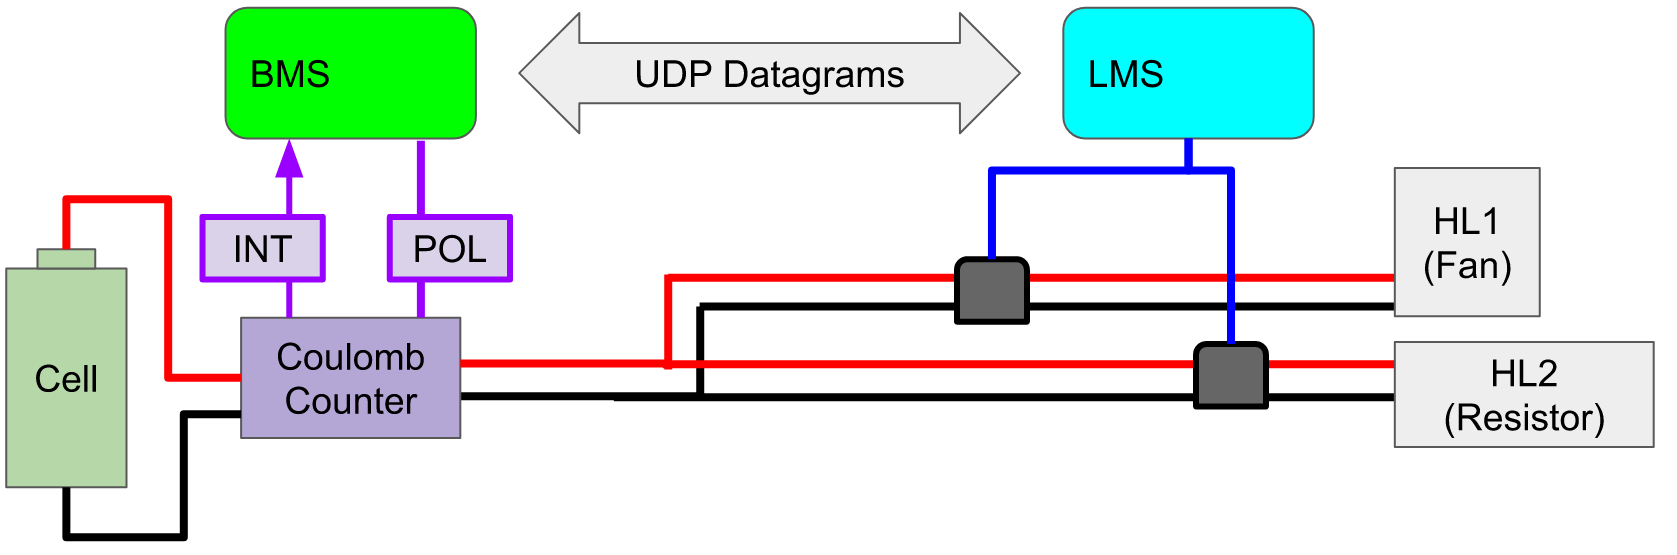
\includegraphics[width=6.5in]{img/uBmsModel.png}
    \caption{BMS and LMS Schematic}
    \label{fig:bmsModel}
\end{figure}
\clearpage
\subsection{Battery Management System Architecture}
In the implementation, the BMS is a Raspberry Pi Zero W \cite{rpiZeroW} which is connected to an LTC4150 Coulomb Counter breakout board.
Figure \ref{fig:coulombCounter} depicts the LTC4150 Coulomb Counter breakout board and its pin names.
The LTC4150 Coulomb Counter breakout board is connected to the nickel–metal hydride (NiMH) battery cells pictured in Figure \ref{fig:nimhBatt}.
Each NiMH cell provides 1.2 V and around 1200mAh of charge.
The NiMH configuration for this project was four cells in series bringing the voltage to 4.8V while maintaining 1200mAh of charge.
This battery model is stored in the BMS for use in accepting and rejecting loads that match the battery configuration - as will be discussed later.

The Raspberry Pi Zero W is configured to fire an interrupt service routine (ISR) on each falling edge of the General Purpose Input-Output (GPIO) port connected to the interrupt port (INT) of the LTC4150 Coulomb Counter (see figure for INT pin).
The LTC4150 Coulomb Counter's INT pin voltage falls low (signaling an interrupt) each time 0.614439C flows through the IN pins and out through the OUT pins - in either direction.
The polarity pin (POL) indicates the in which the 0.614439C has traveled.
By sampling the POL pin each time the ISR is fired, the BMS may track the current flow through (and remaining charge in) the monitored battery. 

The BMS, being a Raspberry Pi Zero W, is also equipped with a wireless interface which is used to communicate with the LMS over UDP.
\begin{figure}[!htbp]
    \centering
    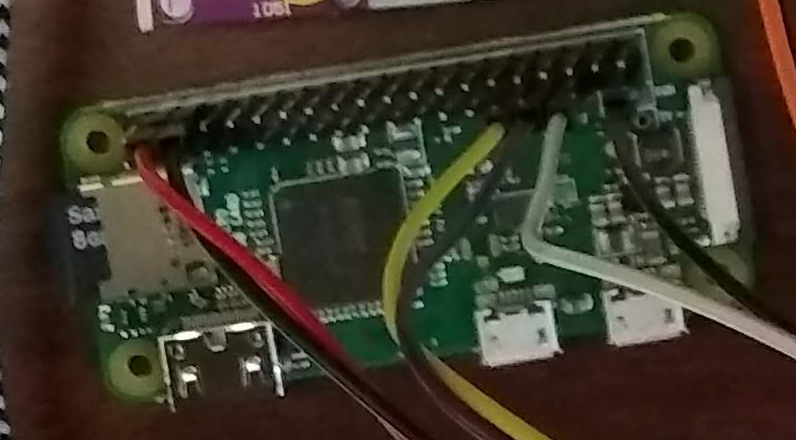
\includegraphics[width=3.5in]{img/rpi0w.png}
    \caption{Raspberry Pi Zero W as a BMS}
    \label{fig:rpi0w}
\end{figure}
\begin{figure}[!htbp]
    \centering
    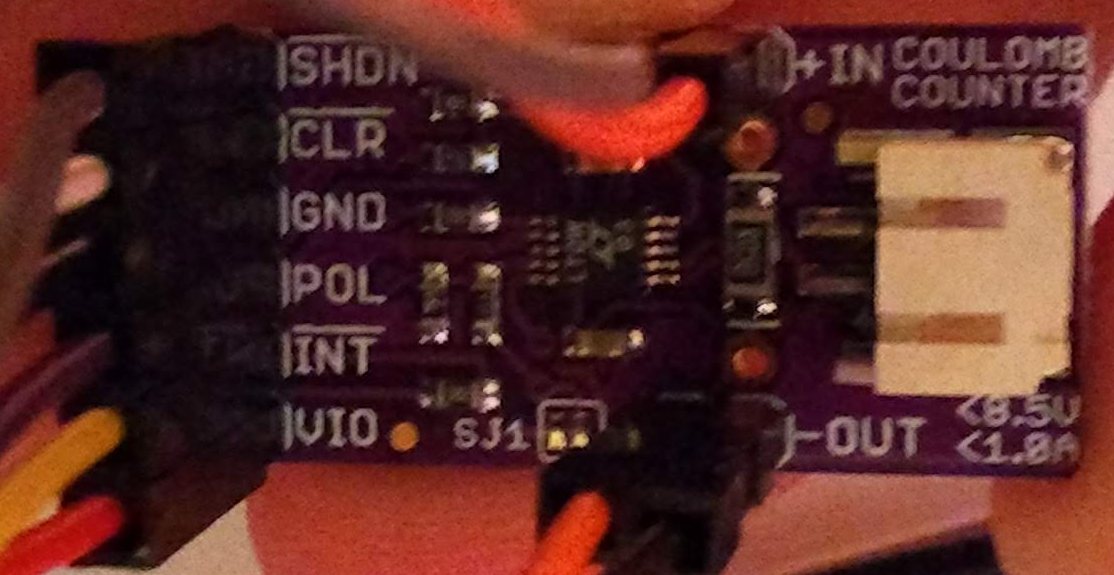
\includegraphics[width=4.5in]{img/coulombCounter.png}
    \caption{An LTC4150 Coulomb Counter Breakout Board}
    \label{fig:coulombCounter}
\end{figure}
\begin{figure}[!htbp]
    \centering
    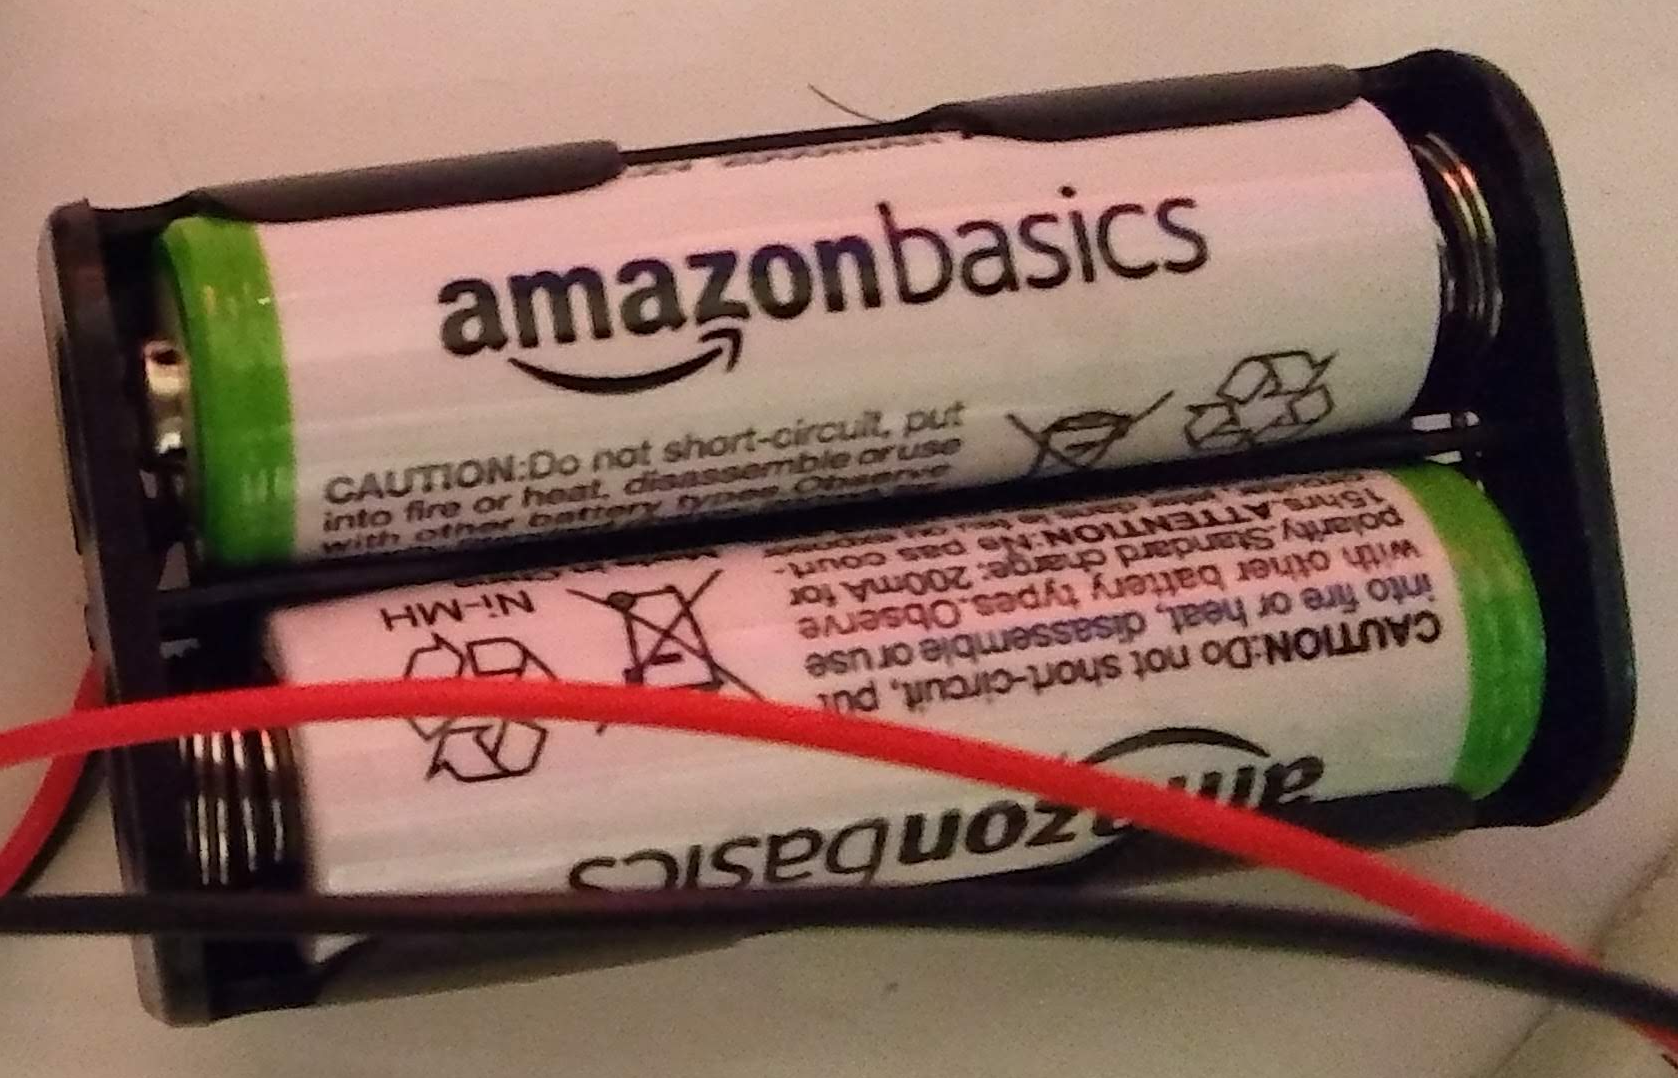
\includegraphics[width=3.5in]{img/nimhBatt.png}
    \caption{1.2V Ni-Mh Batteries}
    \label{fig:nimhBatt}
\end{figure}

\subsection{Load Management System Architecture}
The LMS is a Raspberry Pi 3 which is connected to two PN2222a transistors \cite{pn2222a}.
The first PN2222a transistor, when active, connects the NiMH-supplied power to the 6V 130-size DC motor \cite{130motor}.
The second PN222a transistor, when active, connects the NiMH-supplied power to a 100 Ohm resistor.

The LMS maintains a model of each load and uses these models to request power be supplied by the BMS as will be described later.
The LMS performs all requests over UDP via the built-in Raspberry Pi 3 wireless interface.
Figure \ref{fig:rpi3} shows the Raspberry Pi 3 (LMS), several PN2222a transistors used to activate and deactivate loads, the fan, and several resistors used as loads. The additional resistors and transistors not described here are covered in the Deferred Objectives subsection of Section \ref{sec:discussion}, Discussion.
\begin{figure}[!htbp]
    \centering
    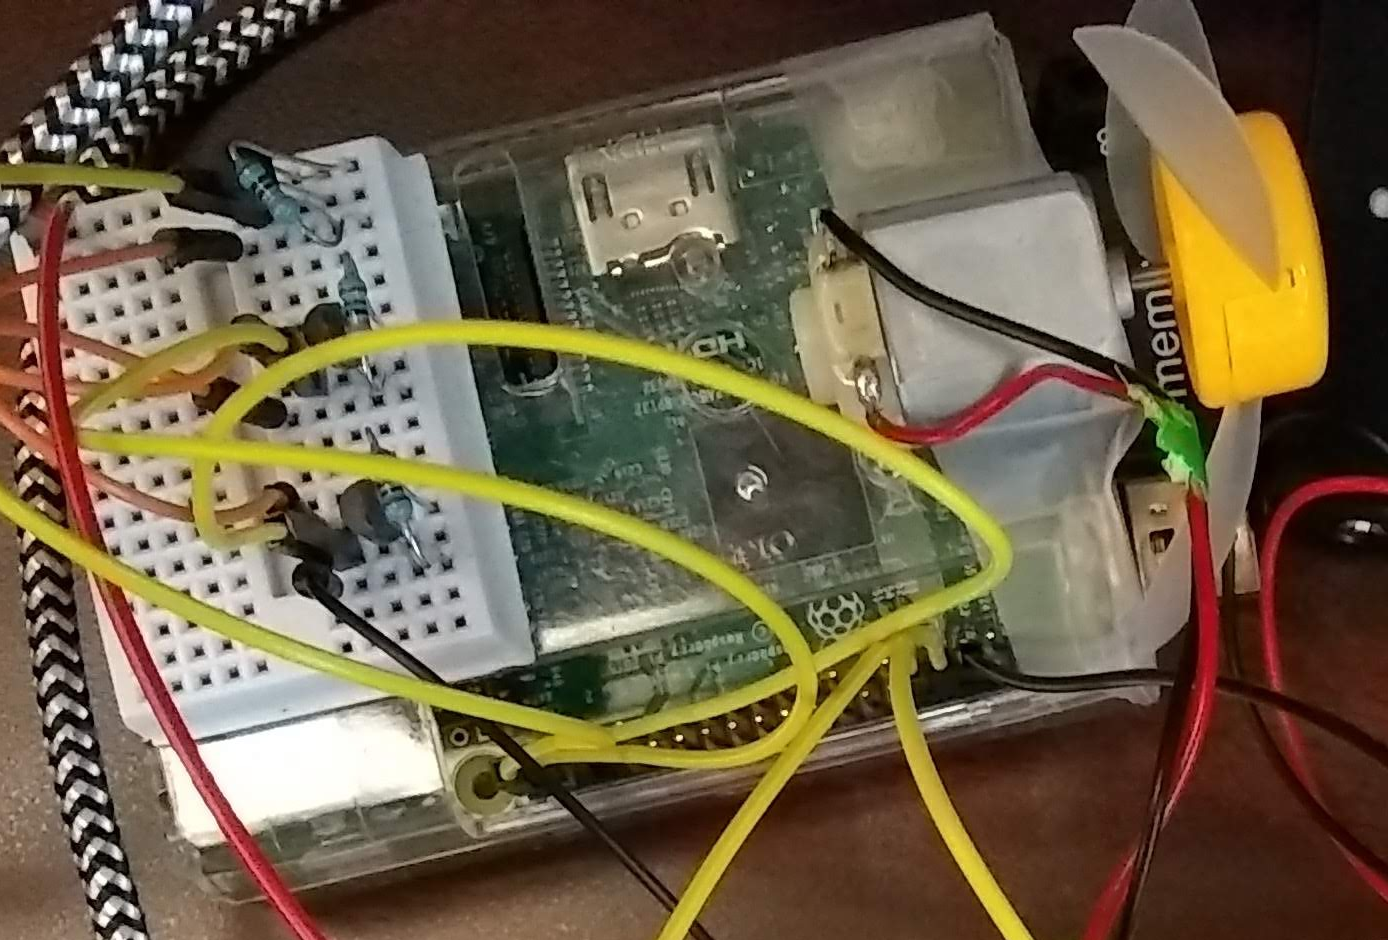
\includegraphics[width=6.5in]{img/rpi3.png}
    \caption{Raspberry Pi 3}
    \label{fig:rpi3}
\end{figure}

\subsection{System Model Summary}
To place all hardware in perspective, Figure \ref{fig:bmsModelPics} shows the photos of each system atop the high-level schematic.
An important difference in the implementation from the schematic presented is that both Raspberry Pis (the BMS and LMS) are powered via their USB power inputs as each Raspberry Pi contains protection circuitry.
Thus, the only loads powered by the NiMH batteries are the fan and 100 Ohm resistor.
\begin{figure}
    \centering
    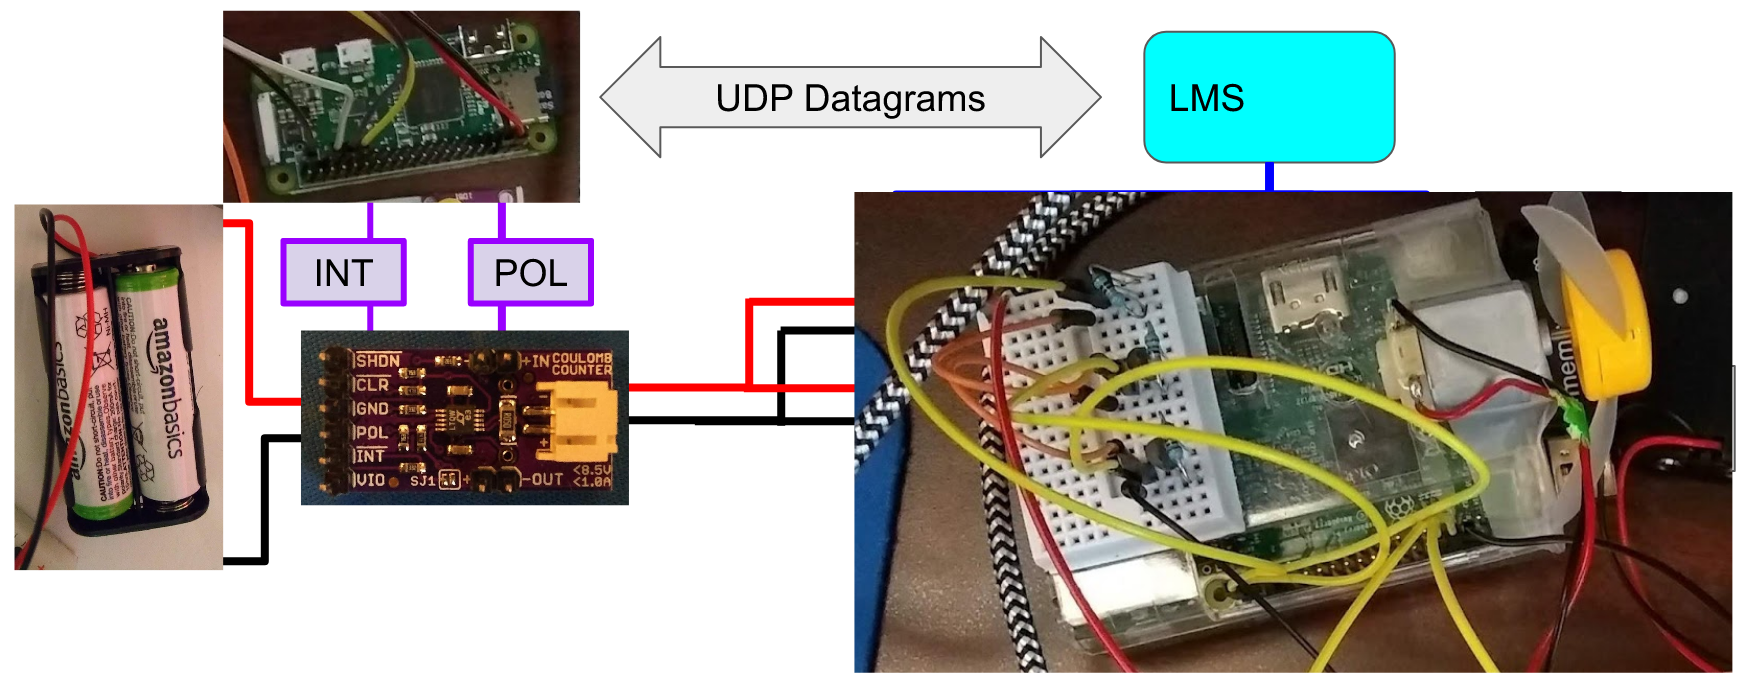
\includegraphics[width=6.5in]{img/uBmsModelPics.png}
    \caption{BMS and LMS Schematic}
    \label{fig:bmsModelPics}
\end{figure}

\section{Request-Based Communication Protocol}\label{sec:rbComm}
Using the hardware presented in the previous section, the BMS and LMS are now capable of describing their respective supplies and demands via the UDP connection.
To facilitate online anomaly detection, the following section describes the protocol used when the LMS intends to activate a load and draw power from the batteries.
The BMS uses this protocol to determine whether supplying electricity for the load is feasible and approves or denies the load as needed.

\subsection{Load Requests}
In practice, components and/or electronic subsystems have a voltage range that can be accepted as input.
Such systems are also bounded in the amount of current they may draw.
This information can be used to model any load in control by the LMS.

Each load in control of the LMS is modeled using the four basic parameters described above: min/max voltage and min/max current.
Together, voltage and current give a min/max power draw for the particular load.
Each load is then transformed into a load request when the following parameters are also specified: release time, duration, deadline, and a unique token.
Release time specifies when the load may become active, duration specifies the maximum time for which the load will be active, and deadline specifies the time by which the load will no longer be active.
Although release time and deadline translate directly to real-time systems, duration may be thought of as worst-case execution time.
The unique token is used as a reference by the BMS and LMS when communicating so the full load request must only be transmitted once and then referred to by the unique token thereafter.

An example load request, constructed as a list of arguments in Python, may look like this:
\begin{lstlisting}
(0,         #Min voltage    (Volts)     (V)
 6,         #Max voltage    (Volts)     (V)
 0,         #Min current    (Amps)      (A)
 0.200,     #Max current    (Amps)      (A)
 0,         #Min Power      (Watts)     (W)
 1.2,       #Max Power      (Watts)     (W)
 10,        #Release time   (seconds)   (s)
 10,        #Duration       (seconds)   (s)
 0,         #Min Energy     (Joules)    (J)
 12,        #Max Energy     (Joules)    (J)
 120,       #Deadline       (seconds)   (s)
 0x0217)    #Unique Token   (hexadecimal)
\end{lstlisting}
which specifies a load with a voltage range of 0-6 volts (V), current range of 0-200 milliamp hours (mAh), power range of 0-1.2 Watts (W), release time of 10 seconds, duration of 10 seconds, energy range of 0-12 Joules (J), a deadline of 120 seconds, and a hexadecimal token 0x0217.

The LMS maintains a dictionary of load requests sent to the BMS which is updated whenever the BMS changes the accepted/rejected status of the request. 

\subsection{Load Request Replies}
Upon receiving a load request from the LMS, the BMS performs several comparisons.
The voltage range of the load is used to determine whether under- or over-voltage constraints apply.
For example, suppose the battery managed by the BMS were reconfigurable as a 12V or 24V battery. One load may require 24V supply while a second load may require a 12V supply. The BMS must either accept both loads at differnt time ranges (so it may reconfigure cells in between) or reject one of the loads.
Supplying 12V to the 24V-only system (or vice-versa) may cause undervoltage (or overvoltage) and damage components.

Similarly, current ranges may be used to determine whether the current battery configuration can support the minimum and maximum current draw expected from the load.
The maximum current draw may be compared against the maximum current output from the present cell configuration.
The minimum current draw will be used later to determine mismatched loads.

The power ranges are used to determine whether the battery configuration can sustain the peak power draw of a combined set of loads.

The energy ranges, like minimum current draw, are used later in anomaly detection.

Finally, the timing constraints are used to calculate the power and energy ranges from the baseline voltage and current ranges.
The timing constraints also allow the BMS to schedule loads which might otherwise be incompatable due to peak power draw.

After determining if the load request can be satisfied, the BMS replies using only the load requests unique token and an error code (if any such error code exists).
No error code (or an error code of 0) indicates the load request is accepted and is scheduled as defined.

\section{Anomaly Detection Methods}\label{sec:anomalyDetection}
Having established the structure of request-based communication between the BMS and LMS, the following section descrtibes the anomly detection methods used by the implementation.

\subsection{BMS Anomalies}
BMSs are responsible for monitoring a number of characteristics. These characteristics include, but are not limited to:
\begin{enumerate}
    \item State of Charge (SoC),
    \item Depth of Discharge (DoD),
    \item configuration,
    \item min/max voltage,
    \item min/max current,
    \item temperature,
    \item number of cycles,
    \item total power delivered,
    \item Open-Circuit Voltage (OCV),
    \item relaxation time, and
    \item communications
\end{enumerate}

It is possible for any combination of these paramters to deviate from expectations.
However, it is unclear how expectations might be established.
For the purpose of this work, we used the BMS modeling of the battery and the LMS modeling of loads (and thus load requests) to establish expectations.
Online anomaly detection, is possible based on the combination of the BMS battery model and LMS load requests.

\subsection{Anomalies Covered}
In this work, the proposed system model addresses five types of anomalies: over/under voltage, over/under current, and load mismatch.

\subsubsection{Over Voltage}
Overvoltage occurs when the voltage supplied to a load exceeds the acceptable maximum input voltage of the load.
For example, using a 12V battery (ex. from an automobile) to directly power a 5V system (ex. a Raspberry Pi) may result in higher current and damage to the powered system.

Any load request whose minimum voltage range exceeds the battery's maximum configurable voltage range is rejected on the basis of overvoltage protection.

\subsubsection{Under Voltage}
Undervoltage occurs when the voltage supplied to a load falls below the accpetable minimum input voltage of the load.
For example, using a ~5V battery system (ex. the one in this model) to directly power an automobile starter motor (typically powered by a 12V lead acid battery), will likely prevent the load from performing properly.
In the worst case, undervoltage may lead to damage if unprotected field-effect transistors are used.

\subsubsection{Over Current}
Overcurrent occurs when the current drawn by a load exceeds the maximum current for which the load is rated.
For example, suppose a phone charger is rated to draw at most 2.1A while charging.
If the charger were to begin drawing 5.0A, one might suspect a fault in the charger or overvoltage at the supply.
In either case, the result is out of the load specification and may be treated as a short-circuit.

\subsubsection{Under Current}
Undercurrent occurs when the current drawn by a load falls below the minimum current the load is expected to draw.
For example, 

\subsubsection{Load Mismatch}

\section{Experiments}\label{sec:experiments}
\subsection{Experimental Setup}
\subsection{Experimental Execution}
\subsubsection{Over Voltage}
\subsubsection{Under Voltage}
\subsubsection{Over Current}
\subsubsection{Under Current}
\subsubsection{Load Mismatch}

\section{Results}\label{sec:results}
\subsubsection{Over Voltage}
\subsubsection{Under Voltage}
\subsubsection{Over Current}
\subsubsection{Under Current}
\subsubsection{Load Mismatch}

\section{Discussion}\label{sec:discussion}
\subsection{Model Weaknesses}
\subsubsection{Hardware}
\subsubsection{Networking}
\subsubsection{Anomaly Detection}
\subsection{Implementation Challenges}
\subsubsection{Hardware}
\subsubsection{Software}
\subsection{Deferred Objectives}
\subsubsection{Controller Area Network Communication}
\subsubsection{Min/Max Energy Consumption}
\subsubsection{Peak Shaving via Sliding Windows}

\section{Conclusion and Future Work}\label{sec:conclusion}
\section*{Informal Discussion for Professor Fisher}
\subsection{Coulomb Counters as a Limiting Factor}

\bibliography{uBms}
\bibliographystyle{abbrv}

\end{document}
